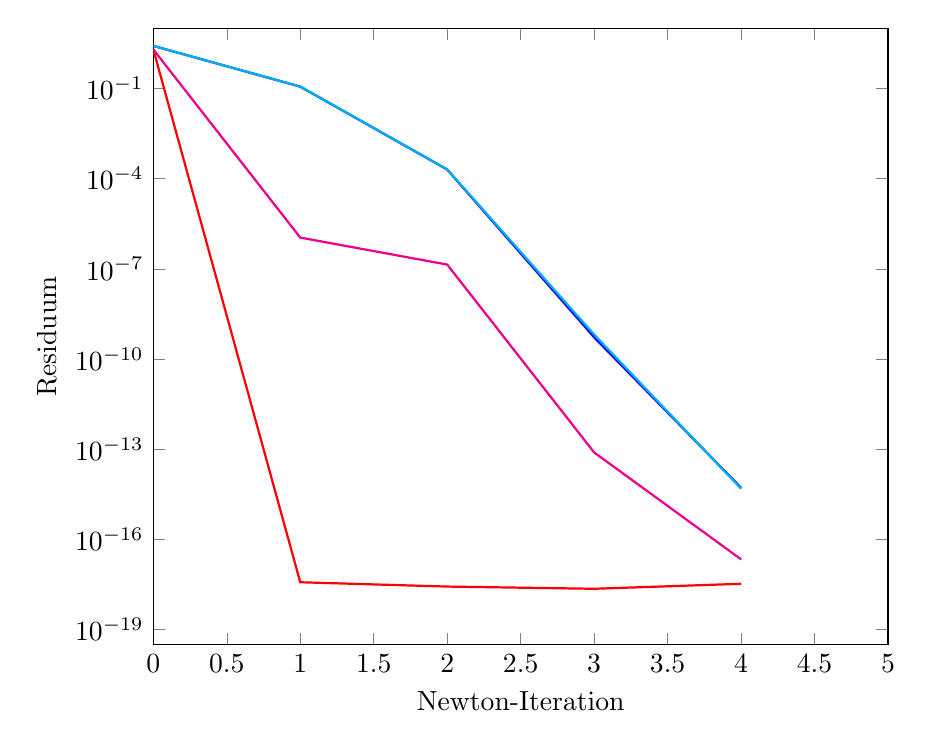
\begin{tikzpicture}[every plot/.append style={thick}] 
\begin{axis}[ 
label style={font=\normalsize}, 
xlabel={Newton-Iteration}, 
ylabel={Residuum}, 
xmin=0, xmax=5, 
ymode=log, 
ymin=0, ymax=10, 
width=0.9\textwidth, 
grid style=dashed, 
] 
\addplot[ 
color=blue, 
] 
coordinates { 
(0, 2.59e+00)(1, 1.14e-01)(2, 2.00e-04)(3, 5.25e-10)(4, 5.21e-15)}; 
\addplot[ 
color=red, 
] 
coordinates { 
(0, 1.97e+00)(1, 3.76e-18)(2, 2.70e-18)(3, 2.28e-18)(4, 3.34e-18)}; 
\addplot[ 
color=cyan, 
] 
coordinates { 
(0, 2.58e+00)(1, 1.15e-01)(2, 2.02e-04)(3, 6.51e-10)(4, 4.85e-15)}; 
\addplot[ 
color=magenta, 
] 
coordinates { 
(0, 1.97e+00)(1, 1.09e-06)(2, 1.38e-07)(3, 7.80e-14)(4, 2.17e-17)}; 
\end{axis} 
\end{tikzpicture} 
